\chapter{永磁同步电机矢量控制实验}
在掌握永磁同步电机矢量控制基本原理的基础上,搭建了永磁同步电机矢量控制实验平台,并进行实验验证矢量控制算法。本章主要介绍永磁同步电机矢量控制实验平台与实验结果,实验平台基于dSPACE搭建,主要包括有永磁同步电机、变频器、电压电流采样模块、光电转换模块以及驱动器保护卡。
\section{永磁同步电机矢量控制实验平台}

\subsection{dSPACE实时仿真系统}
dSPACE是德国dSPACE公司开发的硬件在环仿真平台,用户通过使用Matlab/Simukink搭建控制算法,一键生成代码,载入dSPACE内置的dsp控制器中,无需编写或只需要编写少量代码,十分快捷方便。利用ControlDesk软件的在线调试功能,用户可以修改算法中的任意变量,无需重新编译载入,此外ControlDesk提供了多种虚拟仪器以及触发功能,可以实时观看算法中任意变量的波形,捕捉动态响应。

电机控制控制器的设计研究是一项比较复杂的工作,往往需要根据实际运行情况调整控制参数。 dSPACE快速控制原型构造简单、通过ControlDesk在线调
试调整参数十分方便,非常适合进行电机控制算法研究工作\upcite{_dspacesvpwm_2015,_dspace_2011}。
\subsection{系统实验平台框图}
如图\ref{fig:system}所示为永磁同步电机矢量控制实验平台框图,通过该框图可知,该矢量控制实验平台硬件主要包括PC机、dSPACE、变频器、直流电源、光电转换卡和电机,软件主要包括Simulink和ControlDesk。
\begin{figure}[H]
	\centering
	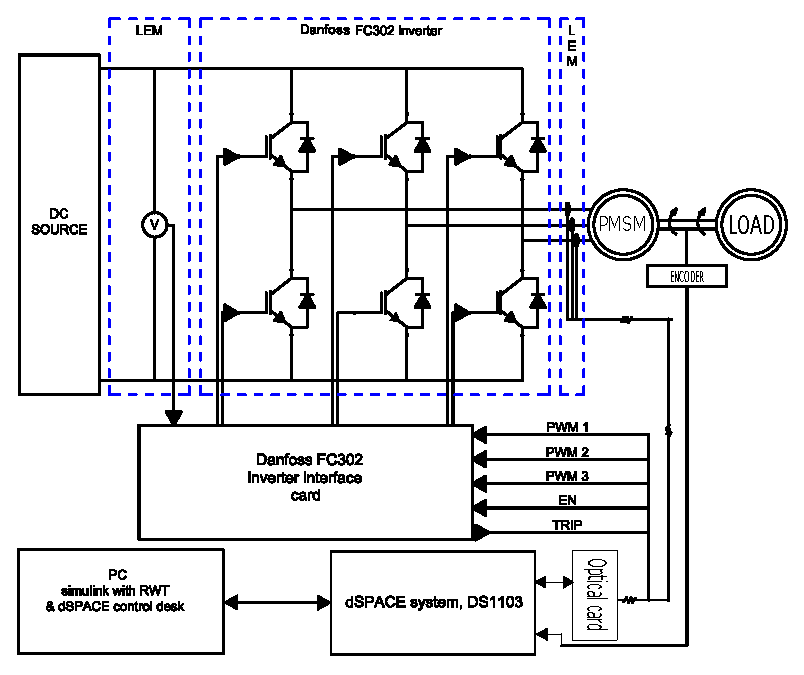
\includegraphics[width=0.7\textwidth]{figs/system.eps}
	\caption{永磁同步电机矢量控制实验平台框图}
	\label{fig:system}
\end{figure}
以下分别介绍永磁同步电机矢量控制实验平台各个组成成分。图\ref{fig:LEMbox}为LEM电流电压采样电路与装上外壳之后的电流电压采样盒,用来采集电机三相电流与变频器直流侧电压,其输出接到dSPACE的ADC采样端口中。
\begin{figure} [h]
	\centering%
	\subfloat[电流电压采样板]{%
		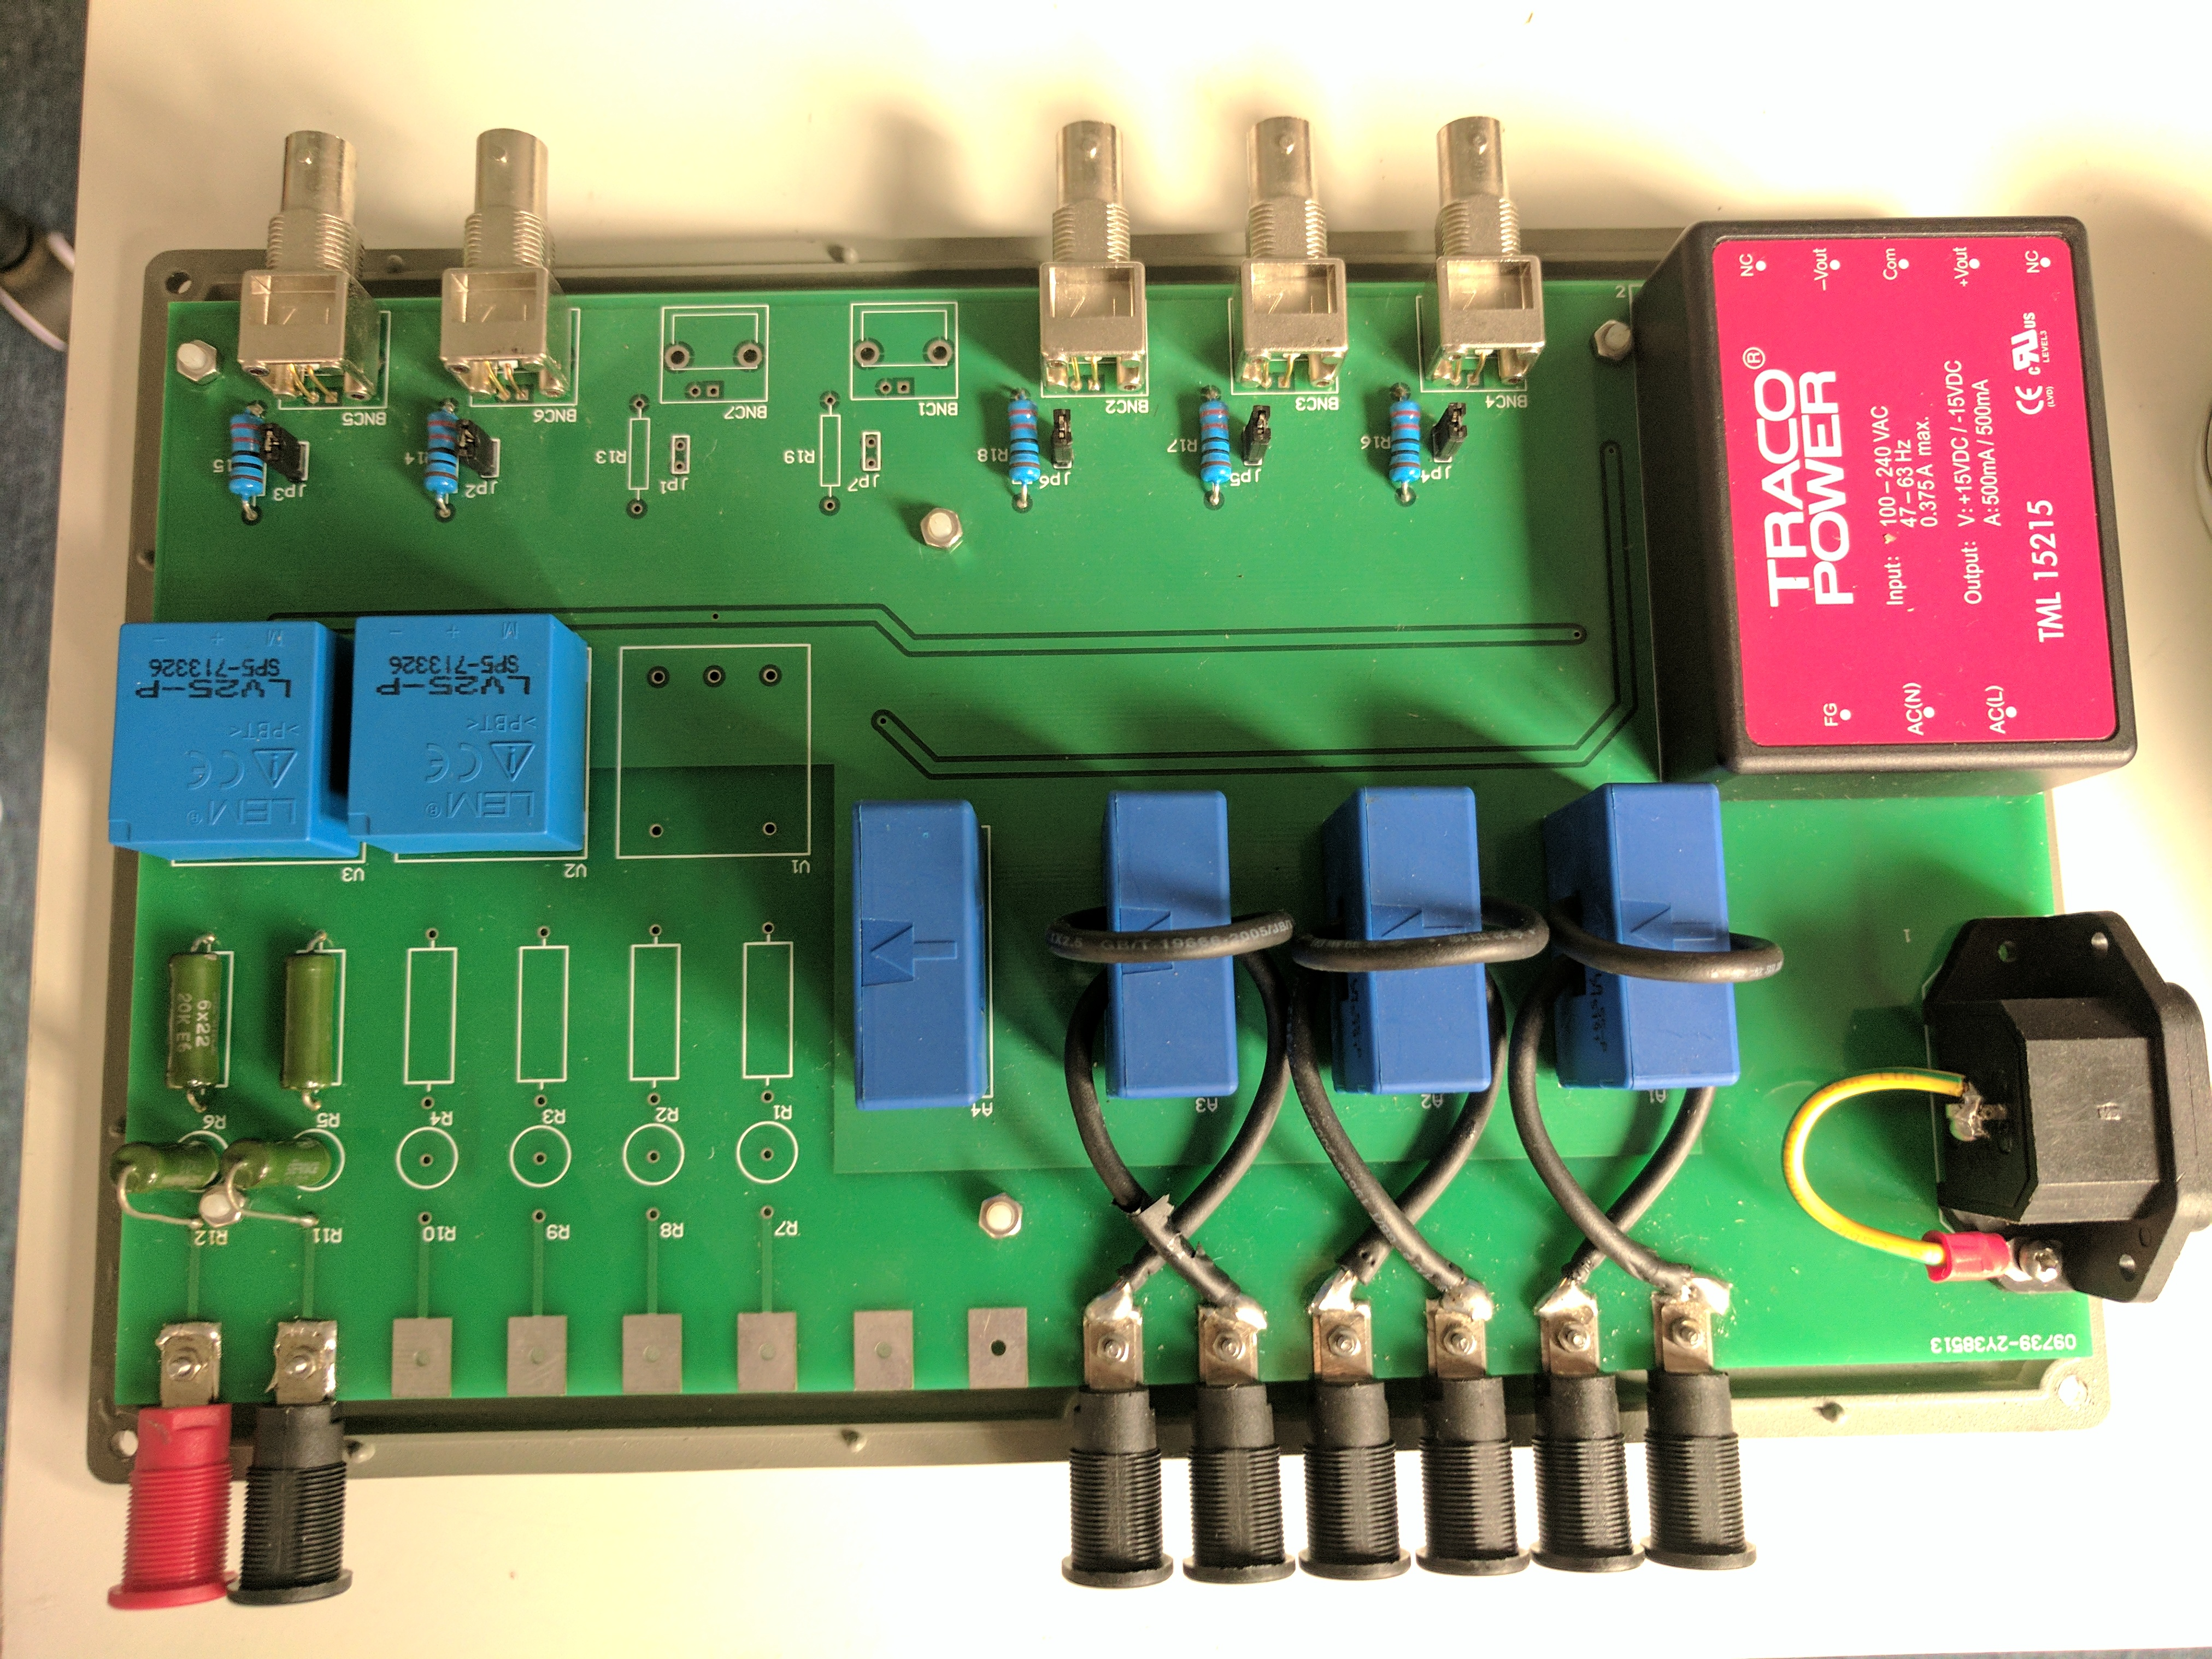
\includegraphics[height=4cm]{figs/LEM.jpg}}\hspace{2em}%
	\subfloat[电流电压采样盒]{%
		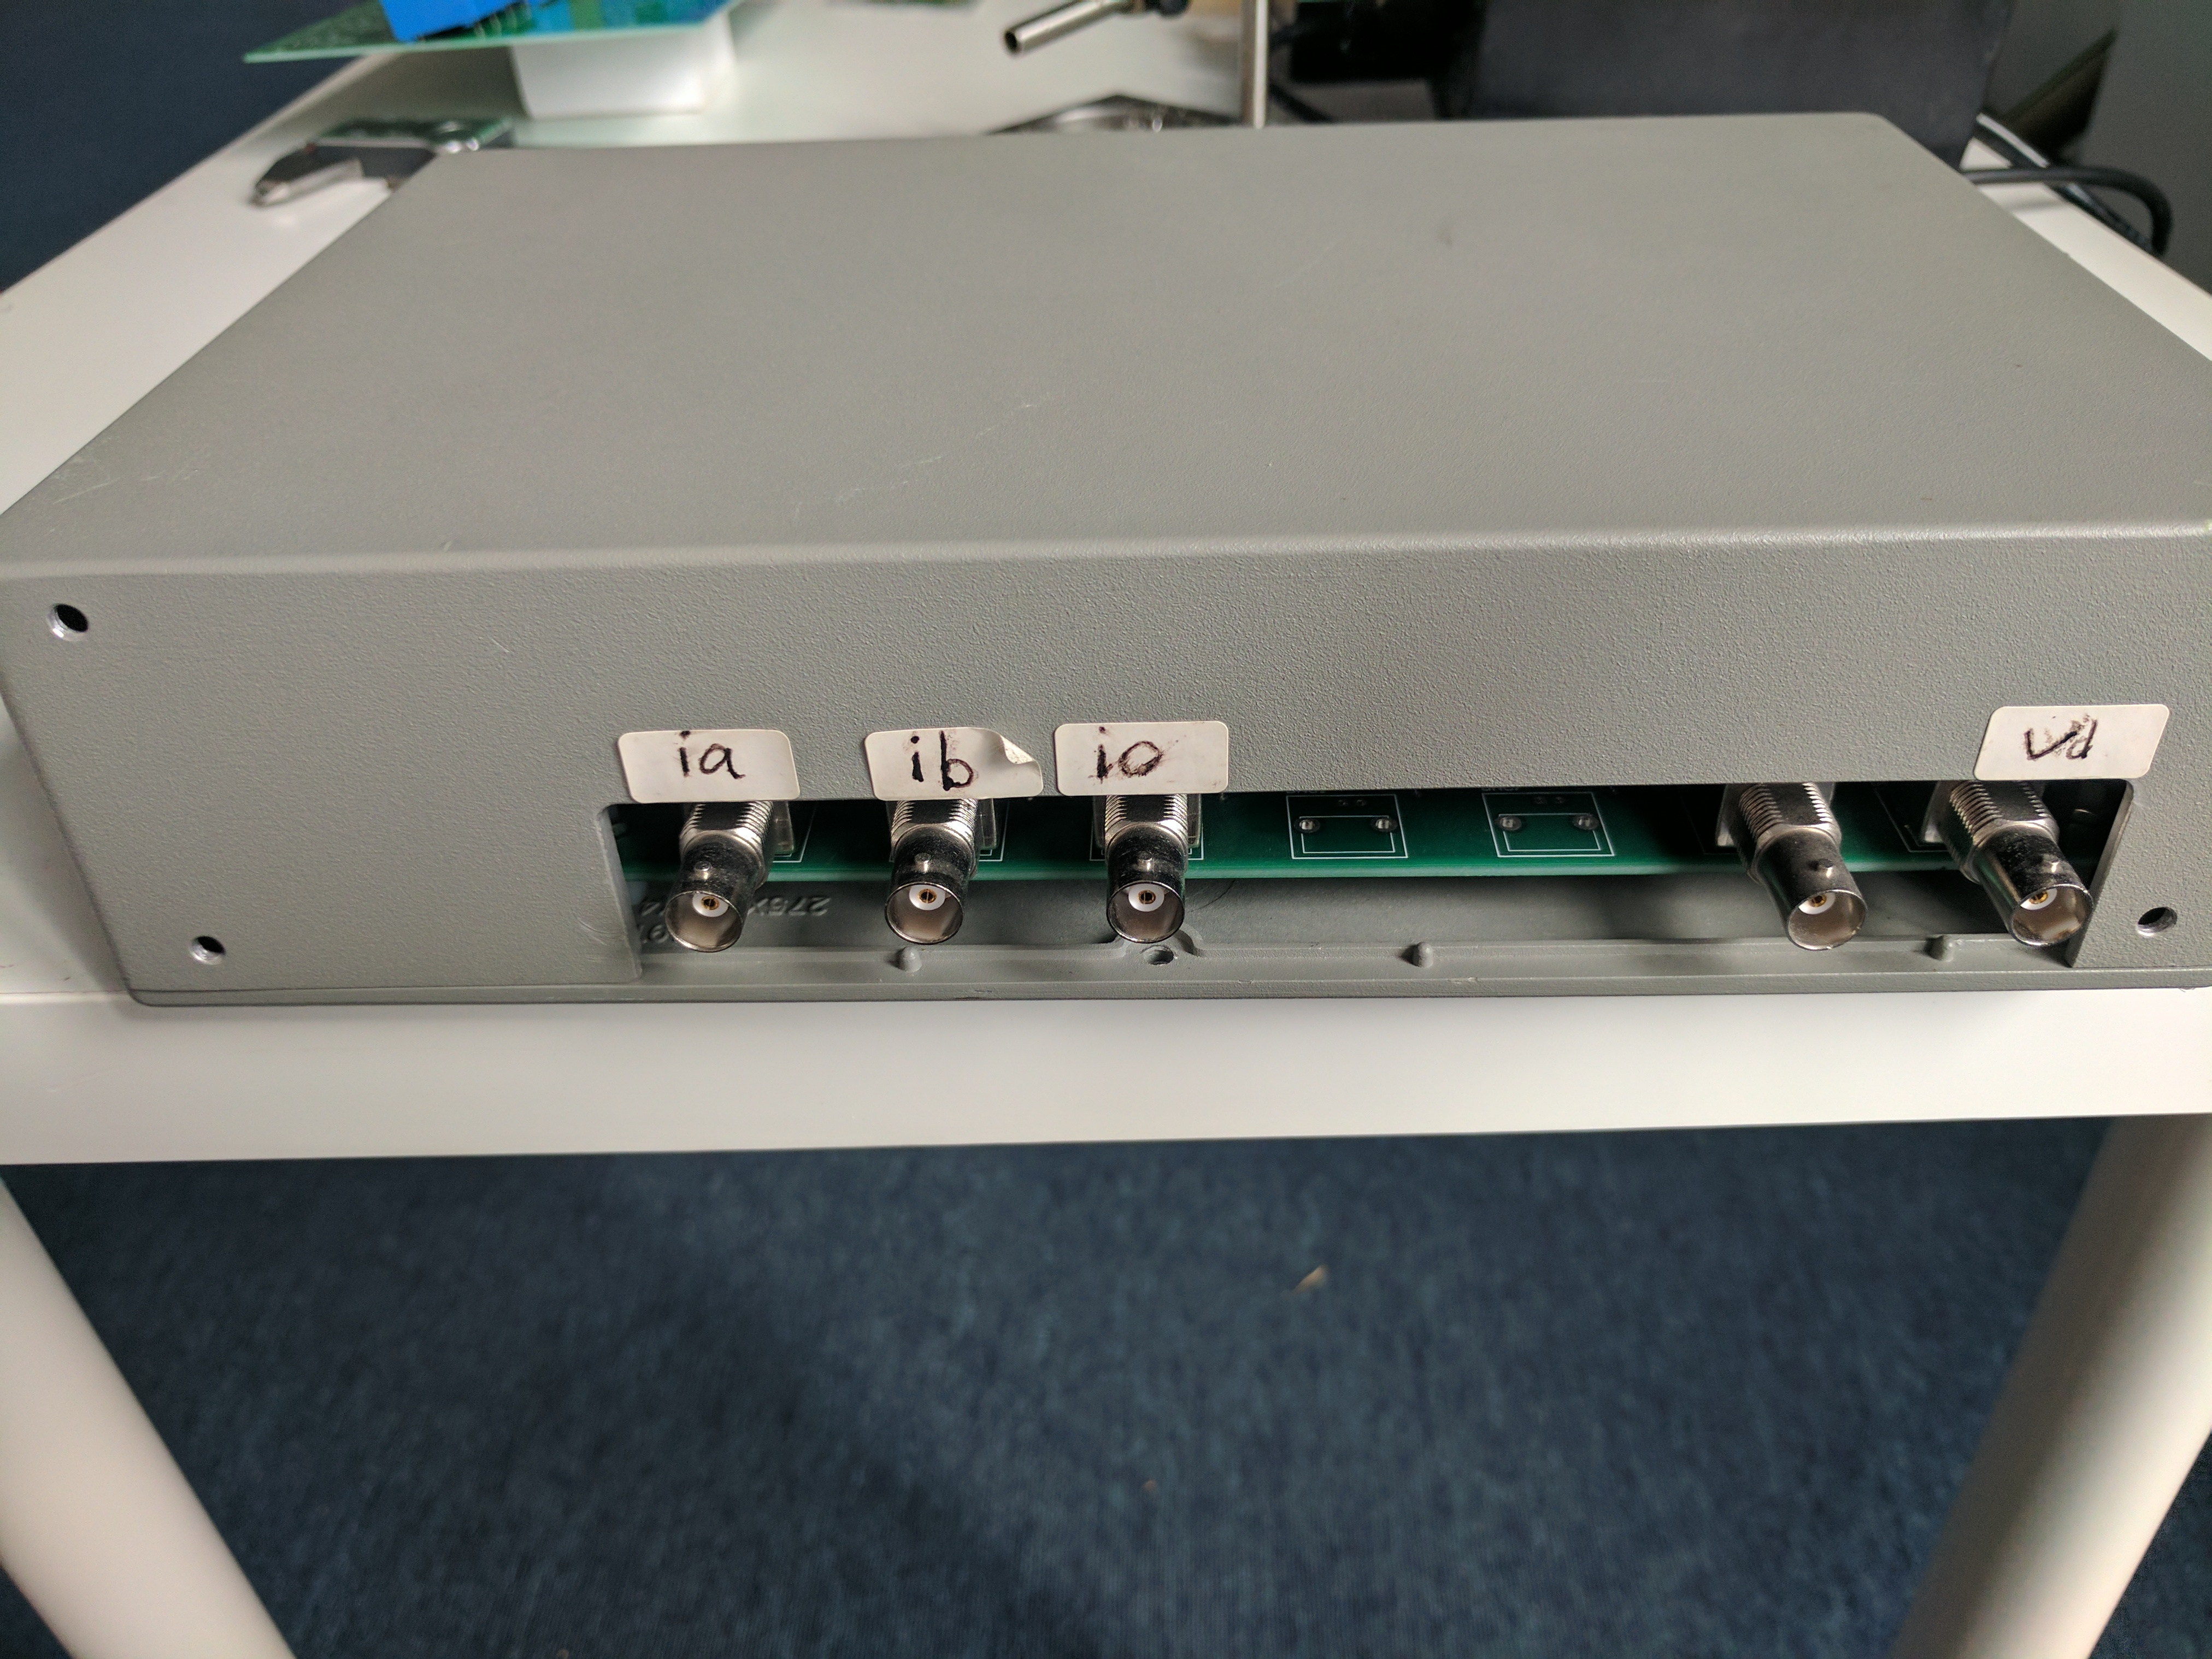
\includegraphics[height=4cm]{figs/LEM_box.jpg}}
	\caption{电流电压采样模块}
	\label{fig:LEMbox}
	\end{figure}
图\ref{fig:optical}为光电转换卡,dSPACE输出的控制信号为电信号,经过光电转换卡转化为光信号传输给变频器接口卡,变频器接口卡再将光信号转化为电信号实现dSPACE与变频器的电隔离,保护dSPACE在使用过程中不受损。
\begin{figure}[H]
	\centering
	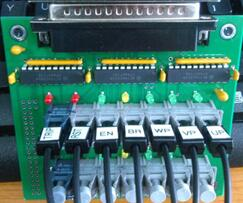
\includegraphics[width=0.7\textwidth]{figs/optical.jpg}
	\caption{光电转换卡}
	\label{fig:optical}
\end{figure}

图\ref{fig:inverter}为安装有定制接口卡IPC3的丹佛斯FC302变频器。IPC3卡能实现FC302变频器三相IGBT桥的控制,具有过流保护、DC侧过电压保护、过频率保护和选择PWM信号死区时间等功能。dSPACE软件保护功能配合IPC3卡的硬件保护功能使得该电机控制实验系统十分安全,调试过程一旦出现过压或者过流,立即会触发保护,变频器立即停止工作。
\begin{figure}[H]
	\centering
	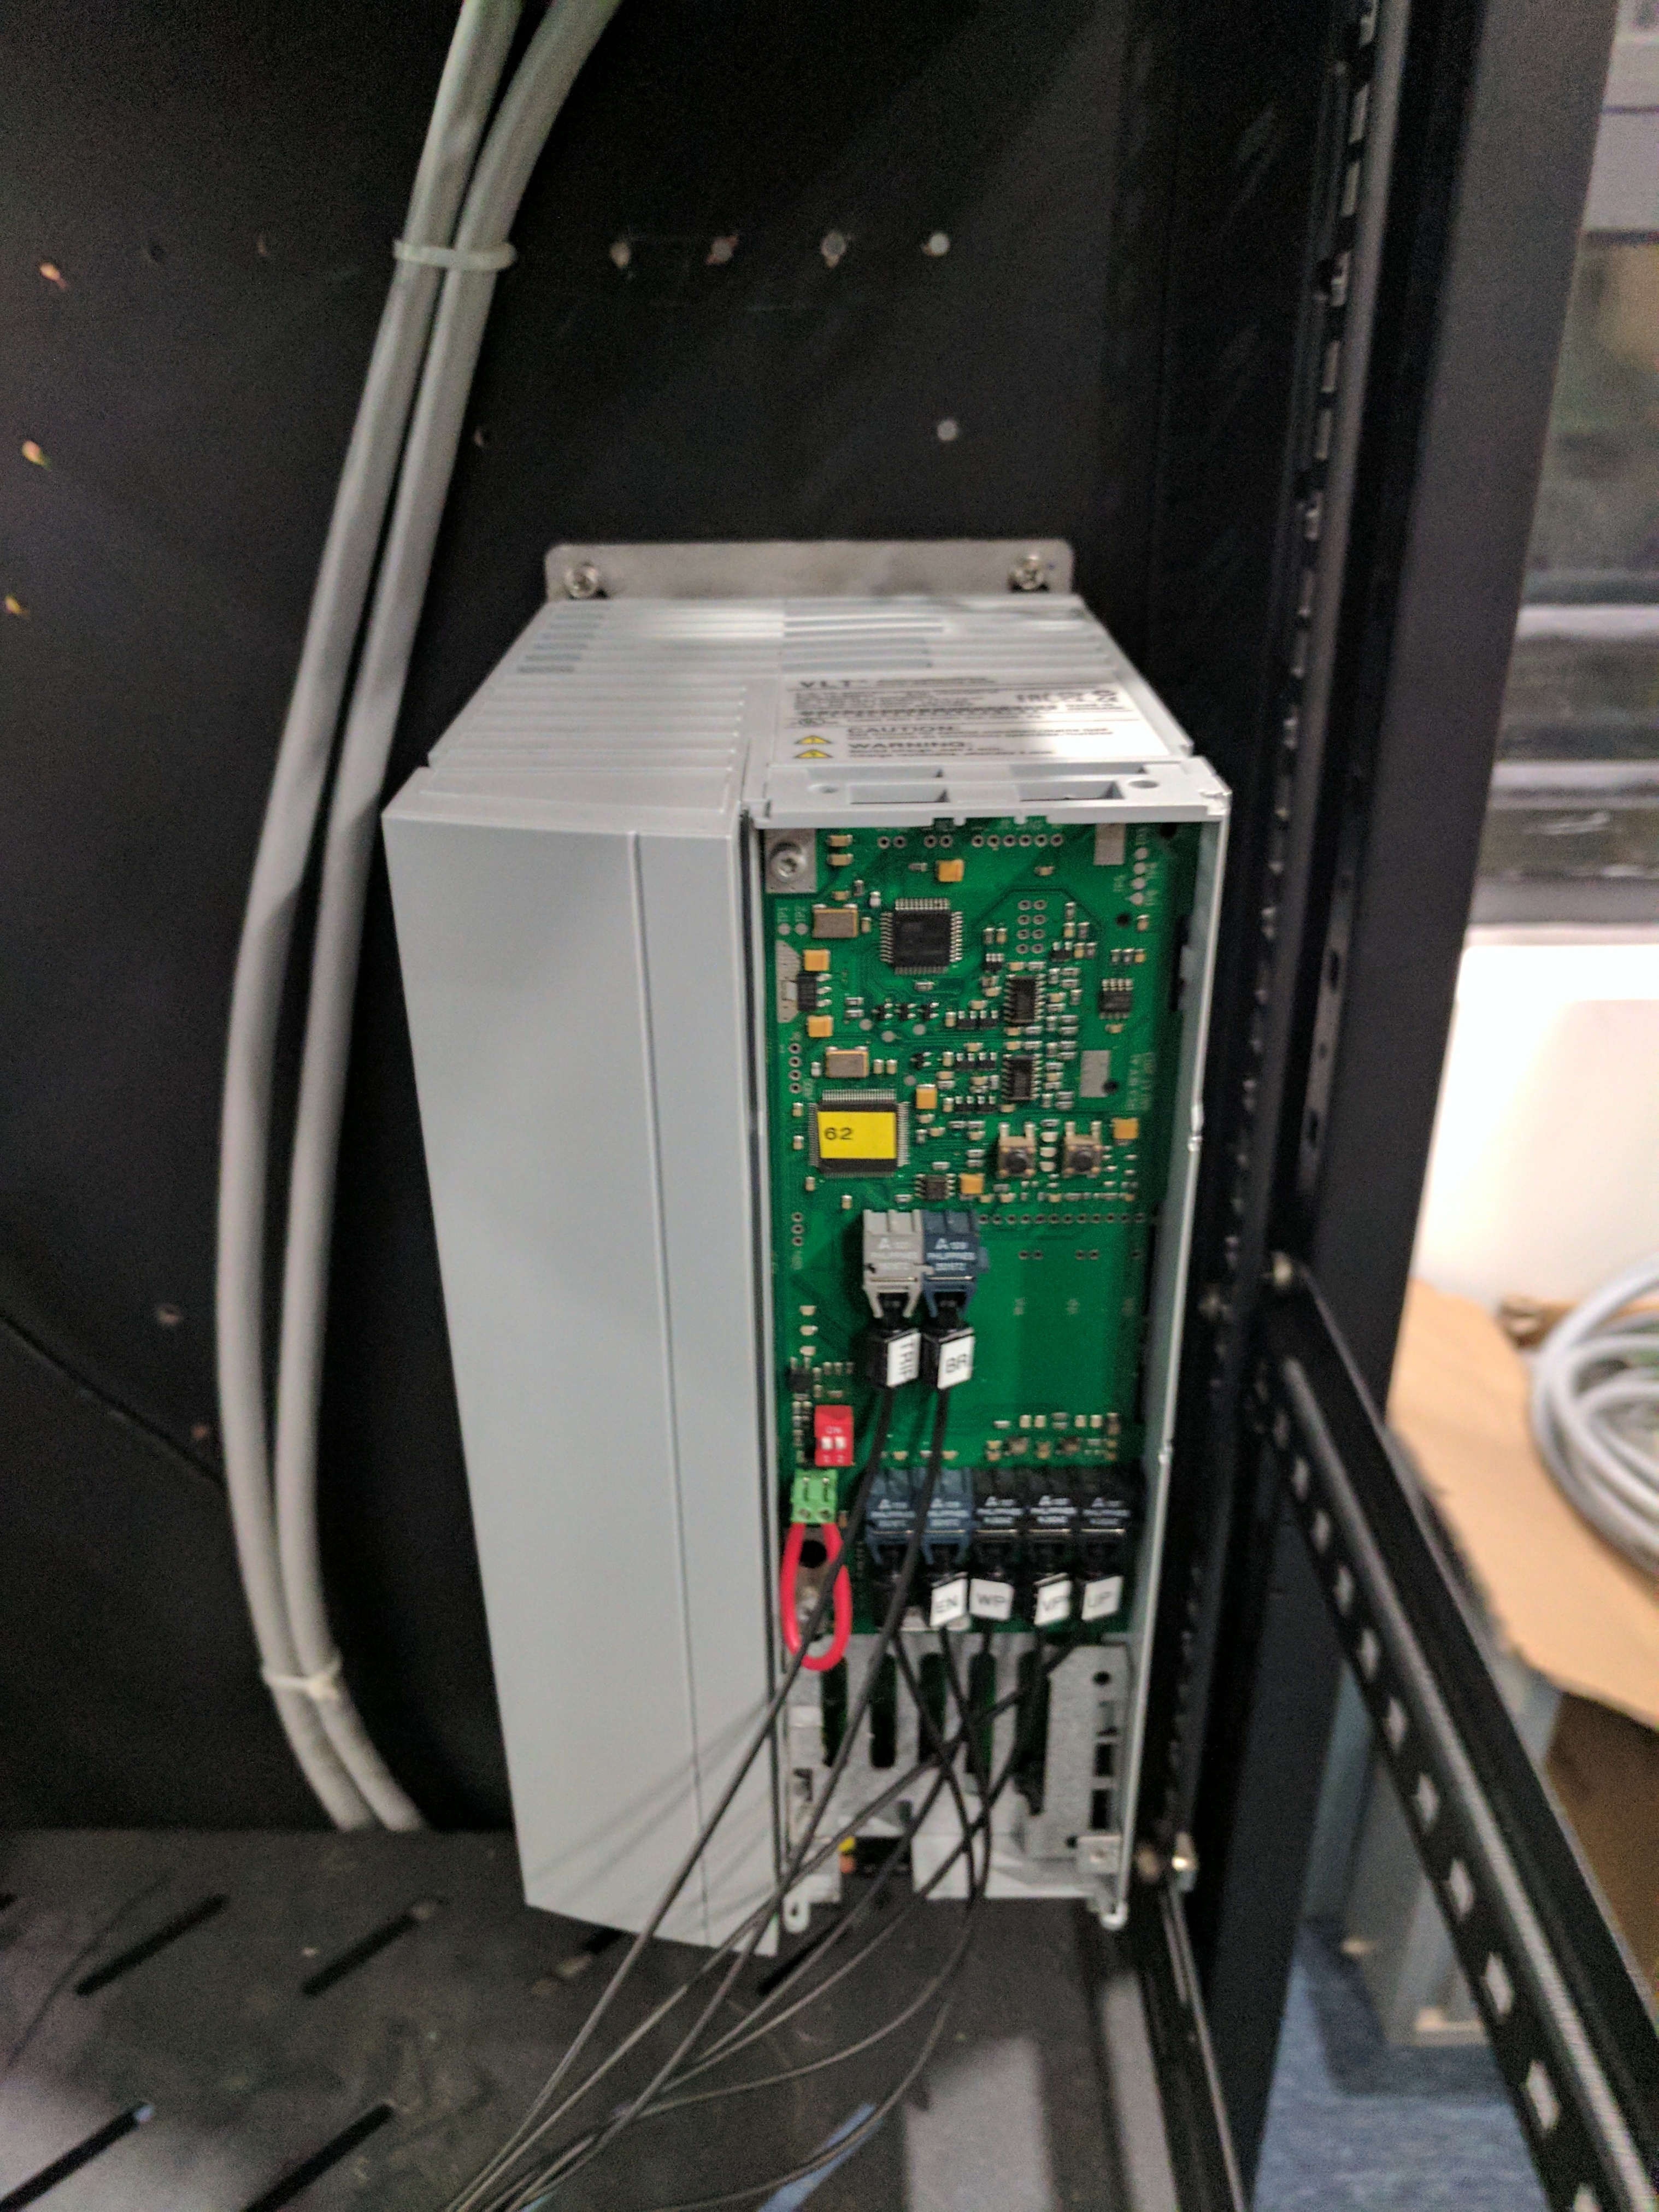
\includegraphics[width=0.7\textwidth]{figs/inverter.jpg}
	\caption{安装有IPC3卡的FC302变频器}
	\label{fig:inverter}
\end{figure}
图\ref{fig:dc_source}为直流电压源其输出接变频器直流电压侧为变频器供电。使用直流源为变频器供电的好处在于直流源输出的电压相对稳定,波动较小,不需要额外电压控制。
\begin{figure}[H]
	\centering
	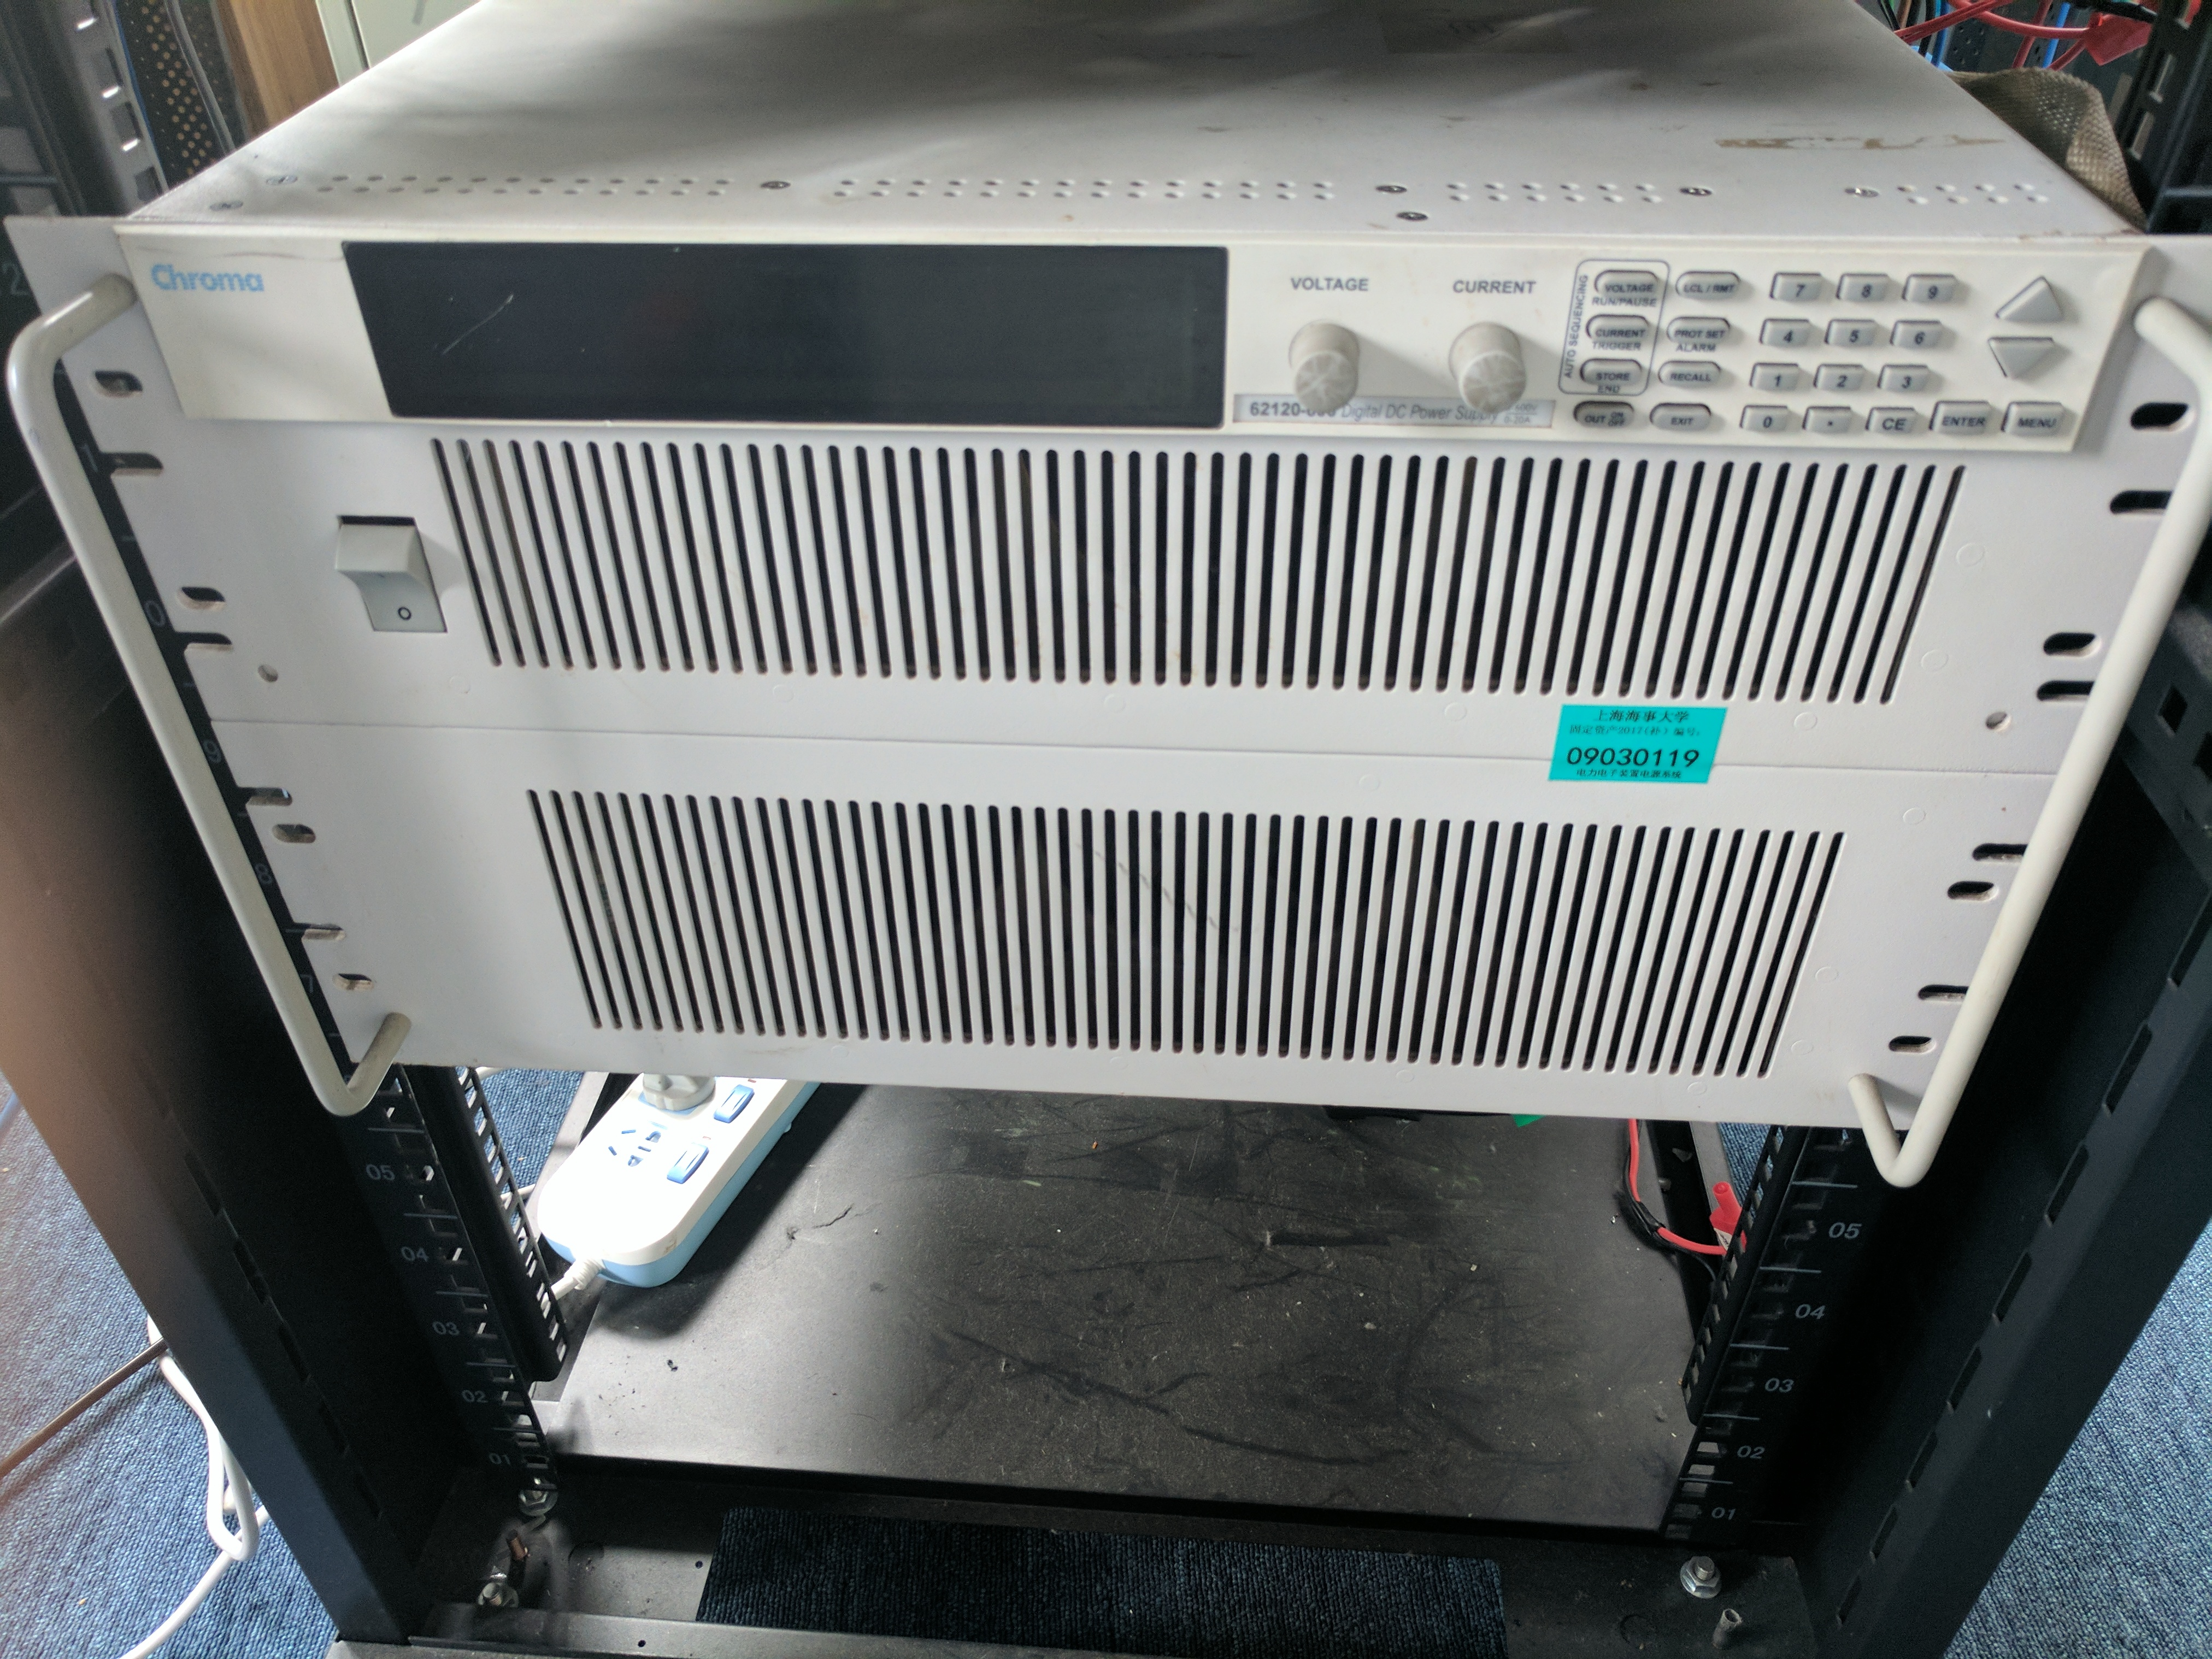
\includegraphics[width=0.7\textwidth]{figs/DC_power.jpg}
	\caption{直流电压源}
	\label{fig:dc_source}
\end{figure}
图\ref{fig:motor}为永磁同步电机与磁力丝杆负载。磁力丝杆\upcite{MLS_for_wave,wang_analysis_2011,holm_design_2013}跟传统的机械丝杆类似,可以实现直线运动和旋转运动相互转换。该系统中永磁同步电机的转子通过齿轮与磁力丝杆的转子相耦合。
\begin{figure}[H]
	\centering
	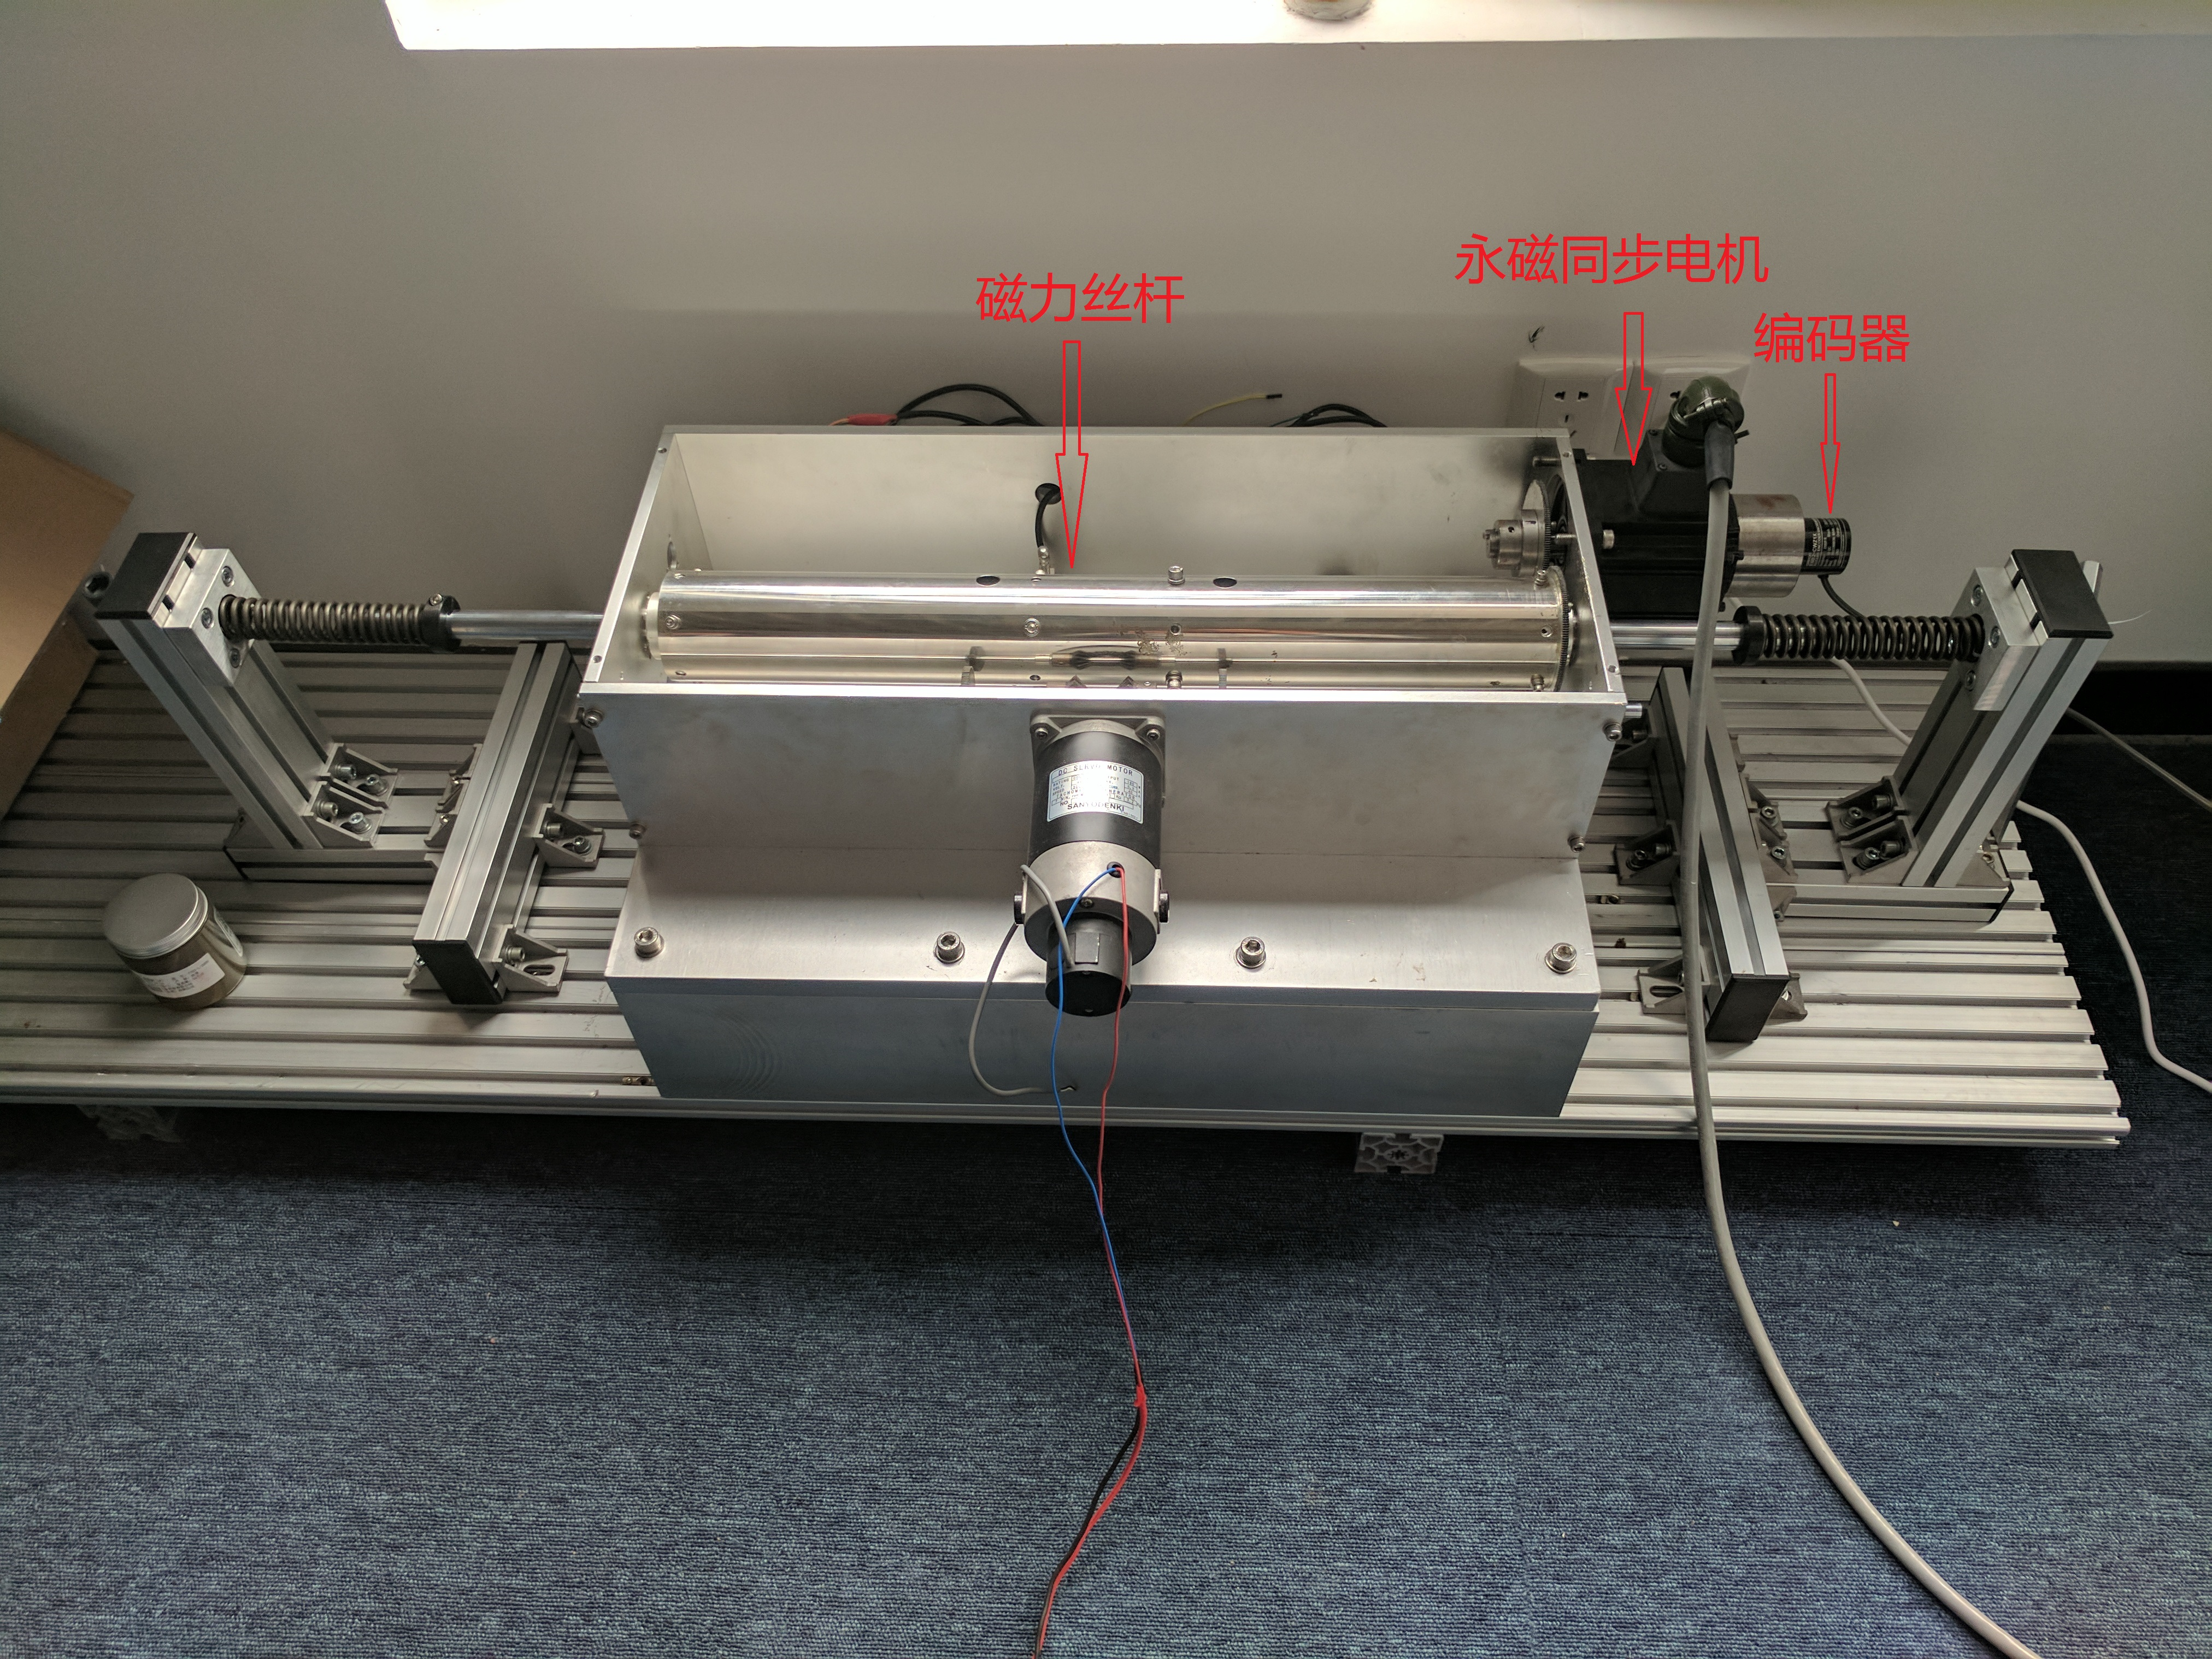
\includegraphics[width=0.7\textwidth]{figs/motor.jpg}
	\caption{永磁同步电机与磁力丝杆负载}
	\label{fig:motor}
\end{figure}
图\ref{fig:ControlDesk}为实验平台ControlDesk在线调试操作界面,通过该界面可以很方便的实时控制系统的启动与停止,在线调节控制器PI参数,显示波形。
\begin{figure}[H]
	\centering
	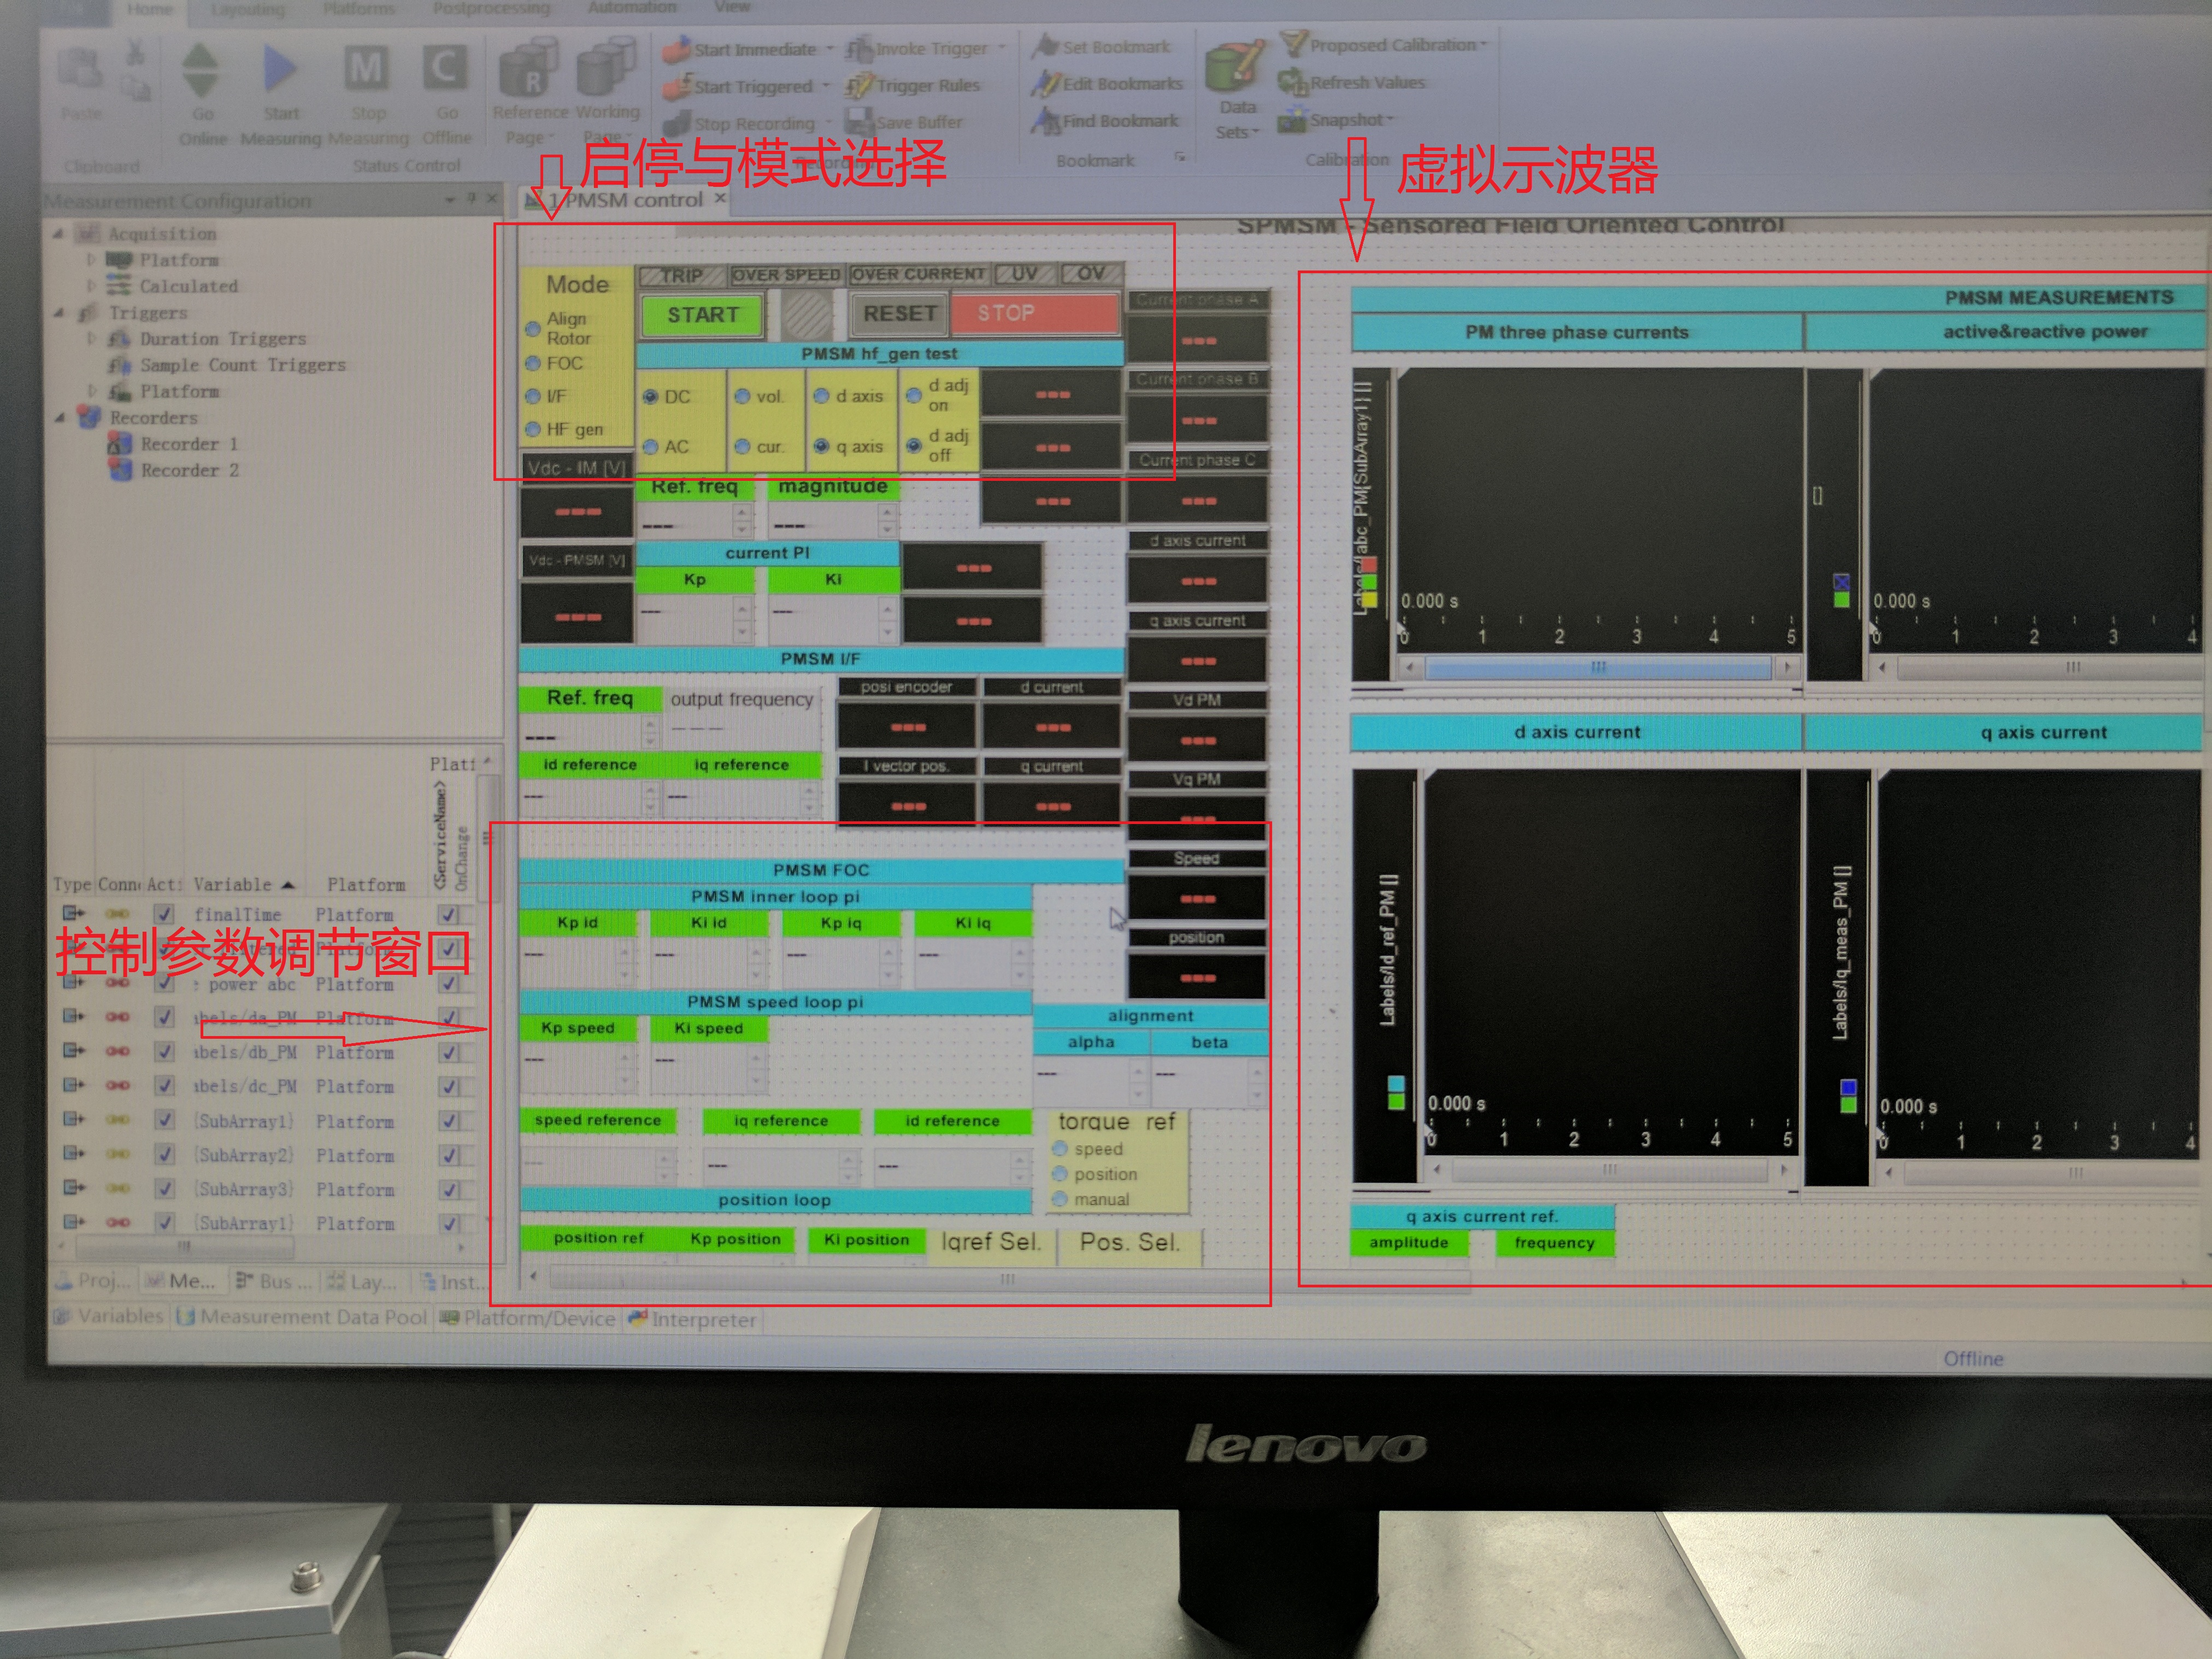
\includegraphics[width=0.7\textwidth]{figs/ControlDesk.jpg}
	\caption{ControlDesk控制界面}
	\label{fig:ControlDesk}
\end{figure}
\section{实验结果分析}
由于实际电机平台的限制,无法控制电机负载。因此,实验只做电机d轴阶跃响应和空载转速控制,并对结果进行分析。
图\ref{fig:d_axis_step}为d轴电流环阶跃响应,d轴PI参数为$K_{p}=5.37$,$K_{i}=1106$,改阶跃响应与第三章分析结果相比,响应比仿真慢。仿真中假设逆变器输出与给定完全一致,但实际逆变器存在死区、非线性等问题,这对电流环阶跃波形有影响。
\begin{figure}[H]
	\centering
	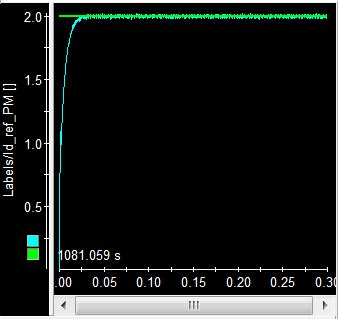
\includegraphics[width=0.7\textwidth]{figs/d_axis_current.jpg}
	\caption{d轴电流阶跃响应}
	\label{fig:d_axis_step}
\end{figure}
\begin{figure}[H]
	\centering
	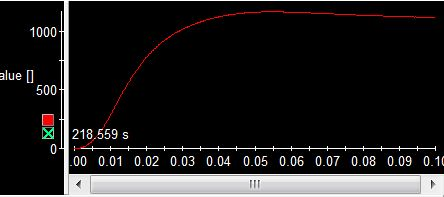
\includegraphics[width=0.7\textwidth]{figs/speed_response.jpg}
	\caption{空载转速响应}
\end{figure}
图\ref{fig:dq_current}为空载运行时,dq电流响应,由该图可知,启动阶段d轴电流存在冲击,这与前面仿真分析类似,是耦合项的影响。
\begin{figure} [H]
	\centering%
	\subfloat[空载d轴电流响应]{%
		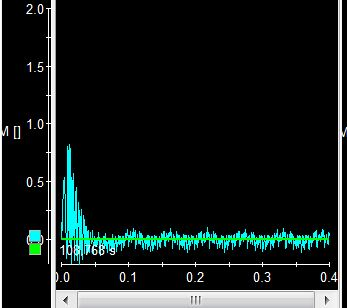
\includegraphics[height=4cm]{figs/d_current_speed_control.jpg}}\hspace{2em}%
	\subfloat[空载q轴电流响应]{%
		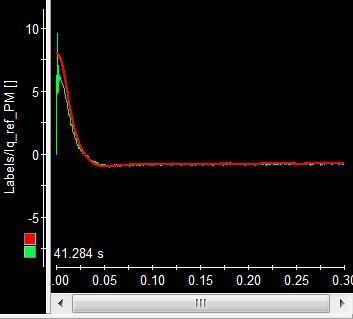
\includegraphics[height=4cm]{figs/q_current_speed.jpg}}
	\caption{空载dq轴电流响应}\label{fig:dq_current}
\end{figure}
\begin{figure}[H]
	\centering
	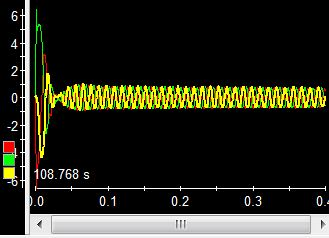
\includegraphics[width=0.7\textwidth]{figs/three_phase_current.jpg}
	\caption{空载abc三相电流}
	%\label{fig:q_response}
\end{figure}
图\ref{fig:estimation}为反电动势位置估算,在启动阶段,转速较低时,估算不准确,0.02s之后,转速较大,位置估算与从编码器获取的位置信号基本重合,与上一章仿真结果吻合。
\begin{figure}[H]
	\centering
	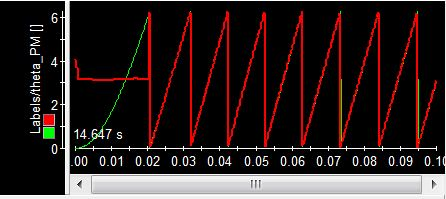
\includegraphics[width=0.7\textwidth]{figs/position_estimation.jpg}
	\caption{反电动势位置估算}
	\label{fig:estimation}
\end{figure}
\ref{fig:ab_flux}为位置估算算法中计算转子位置的$\alpha\beta$磁链,a为带积分漂移的磁链,可以看到积分漂移使得磁链轨迹圆圆心一直在运动,而不在坐标原点。b为漂移补偿后的磁链轨迹,可以看到经过补偿后,磁链轨迹圆为坐标原点。
\begin{figure} [h]
	\centering%
	\subfloat[带积分漂移的$\alpha\beta$磁链]{%
		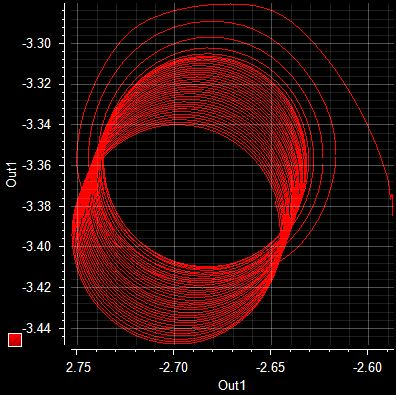
\includegraphics[height=4cm]{figs/flux_with_drift.jpg}}\hspace{2em}%
	\subfloat[漂移补偿后的$\alpha\beta$磁链]{%
		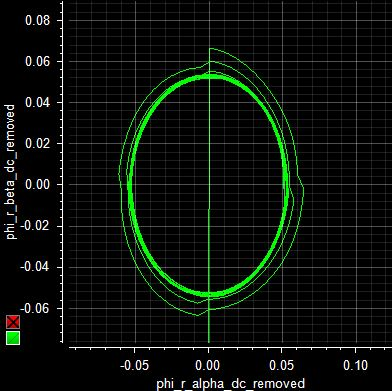
\includegraphics[height=4cm]{figs/flux_with_drift_removed.jpg}}
	\caption{$\alpha\beta$磁链轨迹}\label{fig:ab_flux}
\end{figure}
\section{本章小结}
本章主要介绍了基于dSPACE的矢量控制实验平台的组成以及实验验证结果,对永磁同步电机矢量控制理论研究提供坚实的实验验证。